\documentclass{article}

\usepackage{parskip}
\usepackage[dvipsnames]{xcolor}
\usepackage{textcomp}
\usepackage{hyperref}
\usepackage{listings}
\usepackage{gensymb}
\usepackage{graphicx}
\usepackage{amsmath,amssymb,amsfonts,amsthm}
\newtheorem{lemma}{Lemma}
\usepackage[utf8]{inputenc}
\usepackage{minted}
\lstset{language=c++,breaklines=true}
\lstset{language=C++,
basicstyle=\ttfamily,
keywordstyle=\color{blue}\ttfamily,
stringstyle=\color{red}\ttfamily,
commentstyle=\color{OliveGreen}\ttfamily,
morecomment=[l][\color{magenta}]{\#},
literate=%
{Ö}{{\"O}}1     
{Ä}{{\"A}}1
{Å}{{\AA}}1
{ä}{{\"a}}1
{ö}{{\"o}}1
{å}{{\aa}}1
}

\title{Lösningsförslag Final 2018}
\date{}

\begin{document}

\maketitle

\section*{88-96 poäng}
För att lösa de flesta fallen kan följande insikt användas: i "verkliga" bilder kommer färgerna på samma kolumn inte skilja sig jättemycket en rad ner. Detta kan verifieras med nedanstående exempel.
\begin{figure}[h!]
    \centering
    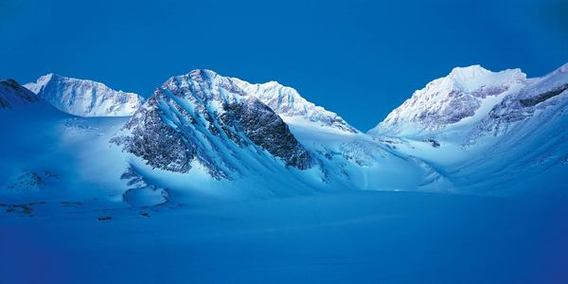
\includegraphics[width=0.7\textwidth]{sample05.jpg}\\
\caption{Sample 5 med originalbredd}
\end{figure}

Om bredden däremot skulle ändras från den originella bredden skulle ett flertal rader skilja sig stort.
\clearpage
\begin{figure}[h!]
    \centering
    \includegraphics[width=0.7\textwidth]{sample5width.png}\\
\caption{Sample 5 med bredd 564 istället för 568}
\end{figure}
Alltså kan en heuristik vara att testa alla rimliga bildbredder ($20-700$), och för varje bredd räkna hur mycket alla rader skiljer sig totalt. Skillnaden mellan två rader kan definieras som \[ \sum_{i=0}^{w} dist(image[row][i], image[row+1][i]) \]  Men hur kan man kvantifiera avståndet mellan två olika färger? Ett sätt som funkar i praktiken är att betrakta färger som en 3d-punkt och mäta avståndet mellan färgerna. Då får vi $dist(a,b)=\sqrt{(a.r-b.r)^2+(a.g-b.g)^2+(a.b-b.b)^2}$. Implementationen av denna algoritmen verkar ge mellan $88$ och $96$ poäng. Svaret blir då det $w$ som får minst totalt avstånd. Denna lösning kan verka köra i kubisk tid, men det är ungefär $O(max_w^2*log(max_w))$. Att visa detta lämnas som en övning till läsaren. Ett tips kan vara att betraka att outputten av följande pythonprogram är ca $nlog(n)$ för en viss bas.

\begin{minted}[fontsize=\small]{python}
n=int(input())
counter=0
for i in range(1,n):
    j=0
    while j<n:
        j+=i
        counter+=1

print(counter)
\end{minted}



\clearpage
\section*{Full poäng}
En bra implementation av ovanstående algoritm ger uppemot 96 poäng, vilket innebär att den endast får fel på ett testfall. Detta testfallet är extremt ondskefullt. Detta beror på att ovanstående heuristik antar att bilden är tagen från en vågrät vinkel. Men vad händer om den är diagonal istället?
\begin{figure}[h!]
    \centering
    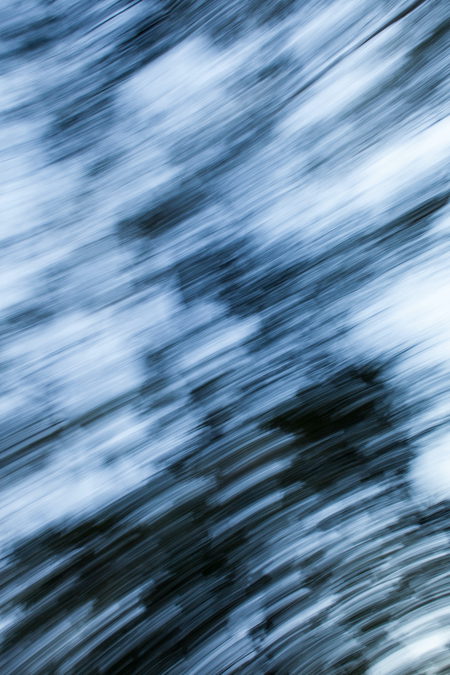
\includegraphics[width=0.5\textwidth]{spinning_fast.png}\\
\caption{En diagonalt lagd bild}
\end{figure}
\\
Här kommer den förra heuristiken uppenbarligen inte funka. För att lösa denna 
krävs en noggrann analys av hur bilderna påverkas om de får fel bredd. För det första visar det sig att den rätta bildstorleken brukar ligga bland toppvalen, med liknande bildbredder bredvid.

\clearpage
\begin{figure}[h!]
    \centering
    \includegraphics[width=0.4\textwidth]{top7.png}\\
\caption{Top 7 valen med ovanstående heuristik. Vänster är totala avstånd, höger är bredd. Rätt bredd är 450}
\end{figure}
\\

Detta ställer då frågan: hur ser de närstende breddarna ut? Nedan visas bilden för breddar 447-453

\begin{figure}[h!]
    \centering
    \includegraphics[width=1\textwidth]{ligma447.png}\\
\caption{w=447}
\end{figure}
\\
\begin{figure}[h!]
    \centering
    \includegraphics[width=1\textwidth]{ligma448.png}\\
\caption{w=448}
\end{figure}
\\
\begin{figure}[h!]
    \centering
    \includegraphics[width=1\textwidth]{ligma449.png}\\
\caption{w=449}
\end{figure}
\\
\begin{figure}[h!]
    \centering
    \includegraphics[width=1\textwidth]{ligma450.png}\\
\caption{w=450}
\end{figure}
\\
\begin{figure}[h!]
    \centering
    \includegraphics[width=1\textwidth]{ligma451.png}\\
\caption{w=451}
\end{figure}
\\
\begin{figure}[h!]
    \centering
    \includegraphics[width=1\textwidth]{ligma452.png}\\
\caption{w=452}
\end{figure}
\\
\clearpage
\begin{figure}[h!]
    \centering
    \includegraphics[width=1\textwidth]{ligma453.png}\\
\caption{w=453}
\end{figure}
\\

Att notera är att det finns en tydlig linje i alla bilder förutom $w=450$, den rätta bredden! Vi kan då uppgradera vår heuristik så att den betraktar både totala färgavståndet och ett numeriskt mått på om bilden innehåller en linje eller inte. Notera att färgerna skiljer sig stort på var sida av linjen. Då kan summan av totala färgavståndet mellan olika sidor av linjerna kvantifiera om en bredd innehåller en linje eller inte. Detta kan implementeras följande i c++: 

\begin{minted}[fontsize=\small]{c++}
vector<pair<double, int>> linescore;
auto getscore = [&](function<int(int)> getindex, function<int(int)> gettarget)
{
    double score = 0;
    int j = 0;
    while (true)
    {
        int idx = getindex(j);
        int target = gettarget(idx);
        if (max(idx,target) >= n) break;
        score += coldist(cols[idx], cols[target]);
        j++;
    }
    return score;
};
rep(i, candidates.size())
{
    int guessWidth = candidates[i];
    double score = 0;

    // -j-1 is right side line, +j is left side
    // distance from true=1
    score += getscore([&](int j) {return guessWidth * (j + 1) + j; },
                      [&](int idx) {return idx + 1; });
    score += getscore([&](int j) {return guessWidth * (j + 1) - j - 1; },
                      [&](int idx) {return idx - 1; });
    // distance from true=2
    score += getscore([&](int j) {return guessWidth * ((j + 2) / 2) - j - 1; },
                      [&](int idx) {return idx - 2 + idx % 2; });
    score += getscore([&](int j) {return guessWidth * ((j + 2) / 2) + j; },
                      [&](int idx) {return idx + 1 + idx % 2; });
    // distance from true=3
    score += getscore([&](int j) {return guessWidth * ((j + 3) / 3) - j - 1; },
                      [&](int idx) {return idx - 3 + idx % 3; });
    score += getscore([&](int j) {return guessWidth * ((j + 3) / 3) + j; },
                      [&](int idx) {return idx + 3 - idx % 3; });
        
    
    linescore.emplace_back(score, guessWidth);
}
\end{minted}

Därefter behöver vi beräkna ett nytt score för varje bild. Om scores är totala färgavståndet radvis och linescore är färgavståndet linjevis kan följande heuristik användas för att kombinera värdena: $newscore[w] = (score[w]/score[0])+(linescore[w]/linescore[0])^{1.7}$. Det är lite sorgligt att behöva inkludera den magiska siffran $1.7$, men det funkar inte för mindre. Det är ändå inte helt orimligt att binärsöka fram siffran. Detta ger nästan fullt poäng, men misslyckas i testfall där bredder långt ifrån svaret får låg score. För att lösa detta väljer vi att bara betrakta de $7$ bredder med lägst värde (detta ger plats för originellbredden $\pm0-3$). Därefter vill vi filtrera ut de som inte hör hemma. För att göra detta hittar beräknar vi för varje bredd summan av avståndet till alla andra bredder. Den bredd som minimerar detta mått blir mittenpunkten. Härifrån betraktar vi bara bredder som ligger 7 ifrån mittenpunkten.

\end{document}